%====================================================================
%====================================================================
\section{Block-models}
%====================================================================
\subsection{Illustration}
\frame{\frametitle{Outline} \tableofcontents[currentsection]}
%====================================================================
\frame{\frametitle{Stochastic block-model for ecological networks} 

  \begin{tabular}{cc}
    \hspace{-.04\textwidth}
    \begin{tabular}{p{.45\textwidth}}
      \paragraph{Data:}
      \begin{itemize}
      \item $n$ species
      \item $Y_{ij} =$ 'intensity' (e.g. count) of the link between species $i$ and $j$
      \end{itemize}
      
      \bigskip \bigskip 
      \paragraph{Adjacency matrix.} \\
      \includegraphics[height=.3\textwidth,width=.3\textwidth]{\fignet/Tree-adjMat}
    \end{tabular}
    &
    \hspace{-.05\textwidth}
    \pause 
    \begin{tabular}{p{.45\textwidth}}
      \paragraph{Stochastic block-model.}
      \begin{itemize}
      \item \bigskip $K$ groups
      \item \bigskip Latent group membership
      $$
      Z_i \sim \Mcal(1, (\pi_1, \dots \pi_K))
      $$
      \item \bigskip Observed count
      $$
      Y_{ij} \sim \Pcal(\exp(\alpha_{Z_i, Z_j}))
      $$
      \item Parameters
      $$
      \theta = (\pi, \alpha)
      $$
      $+ K$
      \end{itemize}

    \end{tabular}
  \end{tabular}

}
  
%====================================================================
\frame{\frametitle{Variational inference} 

  \begin{tabular}{cc}
    \hspace{-.04\textwidth}
    \begin{tabular}{p{.5\textwidth}}
      \paragraph{Conditional distribution.}
      \begin{itemize}
       \item Group memberships:
       $$
       Z_i \independent Z_j
       \qquad \text{but} \qquad 
       Z_i \not\independent Z_j \mid Y_{ij}
       $$
       \item $p_\theta(Z \mid Y)$ is intractable
      \end{itemize}
    \end{tabular}
    &
    \begin{tabular}{p{.3\textwidth}}
      \begin{tabular}{c}
      \begin{tikzpicture}
    \node[hidden] (Z1) at ( 0.0*\edgeunit, -1.2*\edgeunit) {$Z_1$};
  \node[hidden] (Zi) at ( 1.1*\edgeunit,  0.6*\edgeunit) {$Z_i$};
  \node[hidden] (Zn) at (-1.1*\edgeunit,  0.6*\edgeunit) {$Z_n$};
  
  \node[eliminated] (Y1i) at ( 0.8*\edgeunit, -0.5*\edgeunit) {$Y_{1i}$};
  \node[eliminated] (Y1n) at (-0.8*\edgeunit, -0.5*\edgeunit) {$Y_{1n}$};
  \node[eliminated] (Yin) at ( 0.0*\edgeunit,  0.9*\edgeunit) {$Y_{in}$};

  
  \draw[lightedge] (Z1) to (Zi);  
  \draw[lightedge] (Z1) to (Zn);  
  \draw[lightedge] (Zi) to (Zn);  

\end{tikzpicture}

      \end{tabular}
    \end{tabular}
  \end{tabular}
  
  \pause \bigskip \bigskip 
  \paragraph{Variational approximation.} Use a factorable approximate distribution
  $$
  \Qcal = \{ q: 
  \quad q(Z) = \prod_i q_i(Z_i), 
  \quad \underset{\text{no approximation}}{\underbrace{q_i(Z_i) = \Mcal(Z_i; 1, \tau_i)}}
  \}
  $$
  \begin{itemize}
  \item Variational parameters: \qquad $\tau_{ik} \simeq \Pr(Z_i = k \mid Y)$
  \end{itemize}

}
  
%====================================================================
\frame{\frametitle{Variational EM}

  \paragraph{Variational EM algorithm.} {\tt blockmodels} R package \refer{Leg16} 
  \begin{itemize}
  \item \pause \emphase{VE step:} update the \emphase{variational parameters} $\tau_i$ 
  $$
  \tau^{h+1}_{ik} \propto \pi^h_k \prod_{j \neq i} \prod_\ell p_{\theta^h}(Y_{ij} \mid Z_i=k, Z_j=\ell)^{\tau^{h+1}_{j\ell}}
  $$
  \pause \ra Fix-point algorithm
  \item \pause \bigskip \emphase{M step:} update the \emphase{model parameters} $\pi$, $\alpha$
  $$
  \theta^{h+1} = \argmax_\theta \; \Esp_{q^{h+1}} \log p_\theta(Y, Z)
  $$
  \pause \ra Close form for both $\pi^{h+1}$ and $\alpha^{h+1}$
  \end{itemize}
  
  \pause \bigskip \bigskip 
  \paragraph{Model selection.} To choose the number of groups $K$: $vBIC$ or $vICL$ with penalty
  $$
  \text{pen}_{BIC}(\theta) = 
  \underset{\text{node memberships}}{\underbrace{(K - 1) \frac{\log n}{2}}} 
  + \underset{\text{node links}}{\underbrace{\frac{K(K+1)}{2} \frac{\log (n(n-1))}{2}}}
  $$

}


%====================================================================
\frame{\frametitle{A first illustration: Tree species network} 

  \begin{tabular}{cc|c}
    \multicolumn{2}{l|}{\emphase{Simple model: No covariate}} &
    \multicolumn{1}{l}{\onslide+<2>{\emphase{'Validation'}}} \\
    & & \\
    \multicolumn{2}{c|}{{$Y_{ij} \sim \Pcal(\exp(\alpha_{Z_iZ_j}))$}} & 
    \multicolumn{1}{l}{\onslide+<2>{comparison with the}} \\
    & & \multicolumn{1}{l}{\onslide+<2>{phylogenetic classification}} \\
    \multicolumn{2}{l|}{$Y_{ij} =$ number of shared fungal parasites} & \\
    & & \multicolumn{1}{l}{\onslide+<2>{(conipherophyta vs}} \\
    \multicolumn{1}{l}{$\widehat{K}_{ICL} = 7$} & & \multicolumn{1}{l}{\onslide+<2>{magnoliophyta)}}\\ 
    & & \\
    adjacency matrix $Y$ & 
    clustered matrix & 
    \\ 
    \includegraphics[height=.3\textwidth, width=.3\textwidth]{\fignet/Tree-adjMat}
    &
    \includegraphics[height=.3\textwidth, width=.3\textwidth]{\fignet/Tree-adjMat-SBMnull}
    &
    \onslide+<2>{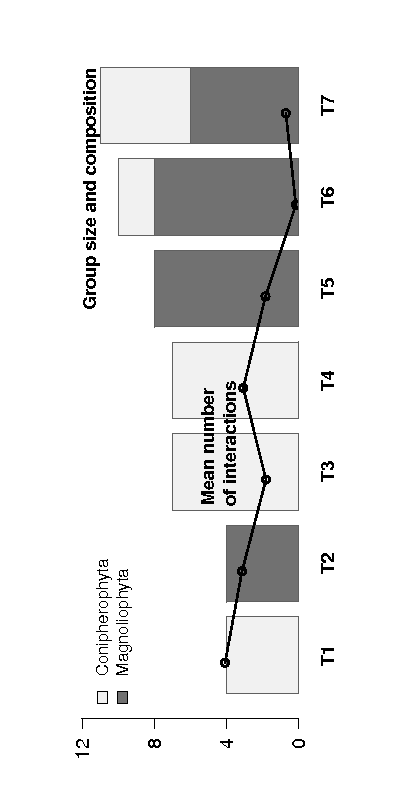
\includegraphics[height=.3\textwidth, width=.3\textwidth, trim=150 150 150 150]{\fignet/MRV10_AoAS_Q7_group}}
  \end{tabular}

}
